%%%%%%%%%%%%%%%%%%%%%%%%%%%%%%%%%%%%%%%%%
% Journal Article
% LaTeX Template
% Version 1.4 (15/5/16)
%
% This template has been downloaded from:
% http://www.LaTeXTemplates.com
%
% Original author:
% Frits Wenneker (http://www.howtotex.com) with extensive modifications by
% Vel (vel@LaTeXTemplates.com)
%
% License:
% CC BY-NC-SA 3.0 (http://creativecommons.org/licenses/by-nc-sa/3.0/)
%%%%%%%%%%%%%%%%%%%%%%%%%%%%%%%%%%%%%%%%%

%----------------------------------------------------------------------------------------
%	PACKAGES AND OTHER DOCUMENT CONFIGURATIONS
%----------------------------------------------------------------------------------------

\documentclass[twoside,twocolumn]{article}

\usepackage{blindtext} % Package to generate dummy text throughout this template

\usepackage[sc]{mathpazo} % Use the Palatino font
\usepackage[T1]{fontenc} % Use 8-bit encoding that has 256 glyphs
\linespread{1.05} % Line spacing - Palatino needs more space between lines
\usepackage{microtype} % Slightly tweak font spacing for aesthetics

\usepackage[german]{babel} % Language hyphenation and typographical rules

\usepackage[hmarginratio=1:1,top=32mm,columnsep=20pt]{geometry} % Document margins
\usepackage[hang, small,labelfont=bf,up,textfont=it,up]{caption} % Custom captions under/above floats in tables or figures
\usepackage{booktabs} % Horizontal rules in tables

\usepackage{lettrine} % The lettrine is the first enlarged letter at the beginning of the text

\usepackage{enumitem} % Customized lists
\setlist[itemize]{noitemsep} % Make itemize lists more compact

\usepackage{abstract} % Allows abstract customization
\renewcommand{\abstractnamefont}{\normalfont\bfseries} % Set the "Abstract" text to bold
\renewcommand{\abstracttextfont}{\normalfont\small\itshape} % Set the abstract itself to small italic text

\usepackage{titlesec} % Allows customization of titles
\renewcommand\thesection{\Roman{section}} % Roman numerals for the sections
\renewcommand\thesubsection{\roman{subsection}} % roman numerals for subsections
\titleformat{\section}[block]{\large\scshape\centering}{\thesection.}{1em}{} % Change the look of the section titles
\titleformat{\subsection}[block]{\large}{\thesubsection.}{1em}{} % Change the look of the section titles

\usepackage{fancyhdr} % Headers and footers
\pagestyle{fancy} % All pages have headers and footers
\fancyhead{} % Blank out the default header
\fancyfoot{} % Blank out the default footer
\fancyhead[C]{Evolutionäre Optimierungsalgorithmen $\bullet$ MK - Einführung in das wissenschaftliche Arbeiten} % Custom header text
\fancyfoot[RO,LE]{\thepage} % Custom footer text

\usepackage{titling} % Customizing the title section

\usepackage{hyperref} % For hyperlinks in the PDF

\newcommand{\e}[1]{\times 10^{#1}}

\usepackage{graphicx}

\usepackage{amsmath}

\usepackage{csquotes}

%----------------------------------------------------------------------------------------
%	TITLE SECTION
%----------------------------------------------------------------------------------------

\setlength{\droptitle}{-4\baselineskip} % Move the title up

\pretitle{\begin{center}\Huge\bfseries} % Article title formatting
\posttitle{\end{center}} % Article title closing formatting
\title{Evolutionäre Optimierungsalgorithmen} % Article title
\author {
	\textsc{Federico Ramírez Villagrana} \\[1ex]
	\normalsize Universität Hamburg \\
	\normalsize Methodenkompetenz - Einführung in das wissenschaftliche Arbeiten \\
	\normalsize Dozent: Dr. Andreas Günther
}
\date{} % Leave empty to omit a date
\renewcommand{\maketitlehookd}{%
\begin{abstract}
\noindent In diesem Paper wird darüber diskutiert, sowohl was Optimierung ist und warum ist es schwer, als auch was evolutionärer Algorithmen (EA) sind und wie, warum,  und wann sind sie hilfreich in dem Optimierung-Bereich. Es wird auch im Detail erklärt, wie EA funktionieren und warum sind sie als teil des künstlichen Intelligenz betrachtet. Es werden auch einige bekannte EA erwähnt und oberflächlich erklärt. Am ende wird darüber diskutiert, was für Vor- und Nachteile die EA haben.
\end{abstract}
}

%----------------------------------------------------------------------------------------

\begin{document}

% Print the title
\maketitle

%----------------------------------------------------------------------------------------
%	ARTICLE CONTENTS
%----------------------------------------------------------------------------------------

\section{Einleitung}

\lettrine[nindent=0em,lines=3]{D} as Problem des Handlungsreisenden (engl. traveling salesman problem oder TSP) ist ein sehr bekanntes und studiertes Problem in dem Informatik-Bereich und es geht wie folgendes:\par
Es muss eine Reihenfolge für den Besuch mehrerer Orte so gewählt sein, dass keine Station außer der ersten mehr als einmal besucht wird, die gesamte Reisestrecke des Handlungsreisenden möglichst kurz, und die erste Station gleich der letzten Station ist. \cite{wiki_tsp}\par
Sei $n$ die Anzahl der Stationen, es gibt $(n-1)!$ mögliche Lösungen für das TSP. Das heißt, dass für $n=4$ es $6$ mögliche Lösungen gibt. Es ist nicht schwer einen brute-force \footnote{Auch Exhaustionsmethode, ist eine Lösungsmethode für Probleme, die auf dem Ausprobieren aller möglichen (oder zumindest vieler möglicher) Fälle beruht. \cite{wiki_brute_force}} Ansatz zu verfolgen für ein Problem, das nur 6 Lösungen hat. Aber wenn $n=50$, gibt es circa $6,1\e{62}$ Lösungen.\par
Folgendes ist hilfreich, um diese Anzahl in einer Perspektive zu setzen: Das Universum ist circa 15 Milliarde Jahre alt, das ist $4,7\e{17}$ Sekunden. Wenn es eine Billion Rechner gäbe, die jede einzeln seit dem Anfang des Universums eine Billion Lösungen pro Sekunde berechnete, bisher wären nur $4,7\e{41}$ Lösungen berechnet worden.\par
Das TSP ist nur ein Beispiel von vielfältigen Probleme, die zu den kombinatorischen Problemen gehören, das heißt, Probleme für die einfach kein brute-force Ansatz möglich ist. Es ist in diesem Fall, dass evolutionärer Algorithmen (EA) hilfreich sind.\par
EA sind ein geeignetes Werkzeug, um gute Lösungen für kombinatorische Probleme zu finden. Natürlich können wir nicht sicher sein, dass wir die beste Lösung gefunden haben, außer wenn wir jede mögliche Lösung berechnen haben. Aber wie es mit dem TSP-Beispiel gezeigt ist, es ist nicht immer möglich, alle mögliche Lösungen (in angemessener Zeit) zu berechnen.

%------------------------------------------------

\section{Stand der Forschung}

\lettrine[nindent=0em,lines=3]{I} n den 70er Jahren wurde erstmals über EA diskutiert. Die erste Form von EA waren die genetische Algorithmen, die in \cite{holland_ga} eingeführt würden. Seit damals wurden jedes Jahr mehrere EA präsentiert. Es ist auch üblich, dass nicht nur Varianten von schon bekannten EA eingeführt werden, sondern auch neue Anwendungen. In \cite{algorithmen_list} allein werden circa 48 EA gelistet.\par
Heutzutage finden sich immer mehr Anwendungen der EA in nahezu allen Bereichen. Von der Medizin \cite{ea_und_medizin} und Biologie \cite{ea_und_biologie} über das Motor- \cite{ea_und_motoren} und Flugzeugdesign \cite{ea_und_flugzeuge_a} \cite{ea_und_flugzeuge_b} bis hin zur Kunst \cite{ea_und_kunst_a} \cite{ea_und_kunst_b} und Wirtschaft \cite{ea_und_wirtschaft}.

%------------------------------------------------

\section{Optimierung}

\lettrine[nindent=0em,lines=3]{I} n dem Mathematik-Bereich, Optimierung bedeutet die Findung von Parametern eines Systems, die ein bestmögliches Ergebnis erzielen. \cite{wiki_optimierung} Wir können diese Findung von Parametern auch wie folgendes definieren: Die Auswahl der bestmöglichen Lösung eines Problems von einer Menge mögliche Lösungen.\par
In Optimierungsprobleme wird eine Zielfunktion (engl. objective function) definiert, die entweder maximiert oder minimiert werden soll. Die Zielfunktion wird \enquote{Kosten-Funktion} oder \enquote{Fitness-Funktion} in Minimierung- und Maximierungsprobleme bzw. genannt.\par
Sei $f(x)$ ein Zielfunktion, $x$ ist ein Vektor und wird \enquote{Entscheidungsvariable} genannt. Die Anzahl von Elementen in $x$ wird die \enquote{Dimension} des Problems genannt.
Die Domäne der Zielfunktion repräsentiert die mögliche Lösungen des Problems. \par
Das Ziel der Optimierung ist es denn, die bestmögliche Lösung des Problems zu finden, das heißt, einen Wert für die Entscheidungsvariable zu finden, sodass die Zielfunktion einen maximal bzw. minimal Wert ergibt.\par
Es gibt verschiedene Klassifizierungen oder Arten von Optimierung:

\begin{itemize}
\item{Eingeschränkt Optimierung.}\\
Die Entscheidungsvariable kann nicht irgendwelchen Wert aus der Domäne der Zielfunktion nehmen. Es gibt Einschränkungen dafür.\\
\item{Multi-objective Optimierung.}\\
Das Problem besteht aus vielfältigen, voneinander unabhängigen Zielfunktionen.\\
\item{Multi-modal Optimierung.}\\
Die Zielfunktion(en) hat/haben mehrere Minima bzw. Maxima. Abbildung \ref{fig:rastrigin} zeigt eine multi-modale Funktion.
\end{itemize}

\begin{figure}[h]
\caption{Rastrigin function. Quelle: \url{https://commons.wikimedia.org/wiki/File:Rastrigin_function.png}}
\label{fig:rastrigin}
\centering
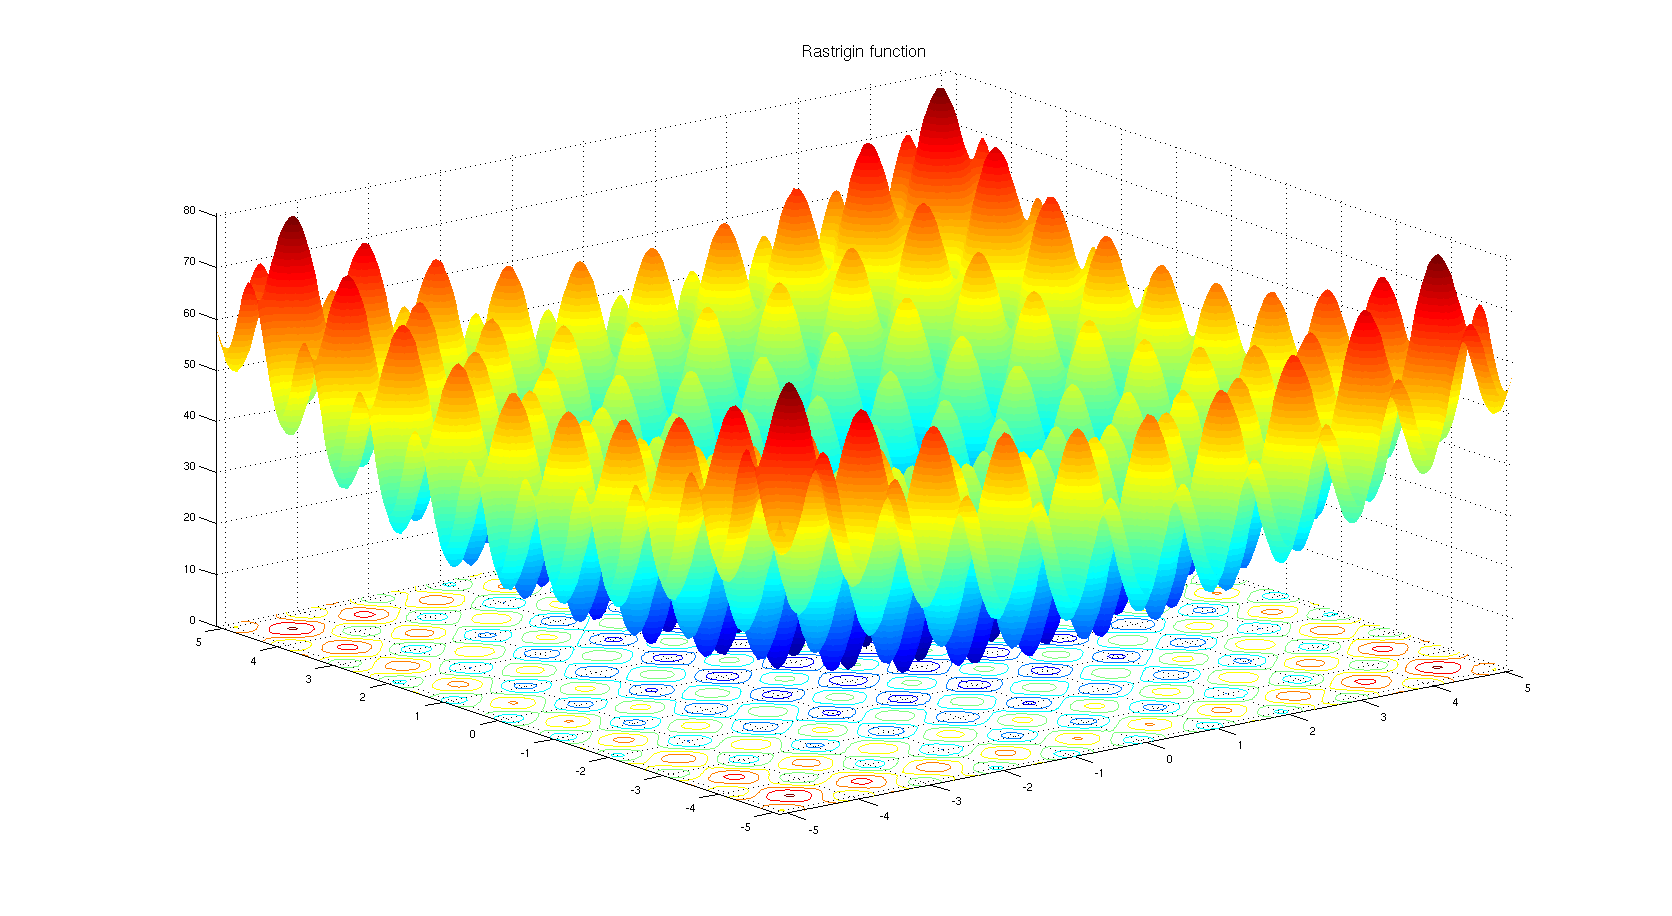
\includegraphics[width=0.5\textwidth]{images/rastrigin_function.png}
\end{figure}

Eine der wichtigsten und schwersten Teile der Optimierung ist es, eine geeignete Zielfunktion zu definieren, die alle die wichtige zu optimieren Faktoren berücksichtigt.
Probleme im wirklichen Leben sind normalerweise eingeschränkt, multi-Objective und multi-modale, oder mit einer hoch Anzahl von Dimensionen. Wegen diesen Eigenschaften der Zielfunktionen und der Optimierungsprobleme ist es schwer eine gute Lösung mittels traditioneller Vorgänge zu finden. Im Laufe der Zeit haben EA sich als gutes Werkzeug zur Lösung dieser Art von Probleme in angemessener Zeit erwiesen.

%------------------------------------------------

\section{Was ist ein evolutionärer Algorithmus?}

\lettrine[nindent=0em,lines=3]{D} er EA-Bereich ist ziemlich neu, deswegen gibt es bisher keine allgemein akzeptierte Definition von evolutionäre Algorithmus.\par
EA sind zwar als Teil des künstliche Intelligenzes (KI) betrachtet, aber genau wo sie in Verbindung mit anderen KI-Methoden stehen, und was der EA-Bereich beinhaltet, ist von dem Autor abhängig. Abbildung \ref{fig:metaheuristics} zeigt eine von mehrere mögliche Klassifikationen von KI-Methoden in Bezug auf Metaheuristics (welche über den Rahmen dieses Papiers hinausgehen).

\begin{figure}[h]
\caption{Klassifikation von Metaheuristics. Quelle: \url{https://en.wikipedia.org/wiki/File:Metaheuristics_classification.svg}}
\label{fig:metaheuristics}
\centering
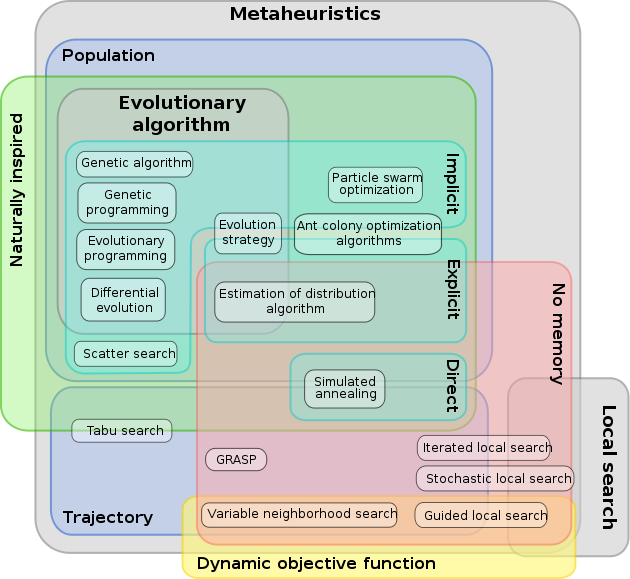
\includegraphics[width=0.5\textwidth]{images/metaheuristics_classification.png}
\end{figure}

In Abbildung \ref{fig:metaheuristics} kann es auch erkannt werden, dass der Autor Particle Swarm Optimization (PSO) und Ant Colony Optimization (ACO) nicht als EA betrachtet, trotzdem gibt es andere Autoren (wie z. B. \cite{wiley_evolutionary}), die diese Algorithmen genau für EA halten.\par

In diesem Paper wird folgende Definition für evolutionärer Algorithmus genommen: Ein Algorithmus, der die Lösung eines Problems durch viele Iterationen entwickelt    .

\subsection{Eigenschaften der evolutionären Algorithmen}
Folgende sind die Hauptmerkmale der EA:

\begin{itemize}
\item{Eine Zielfunktion.}\\
\item{Eine - so genannte - Bevölkerung von mögliche Lösungen.}\\
Eine Menge von Darstellungen der Lösungen (Elemente der Domäne der Zielfunktion) des Problems, die mittels der Algorithmus und mehrere Iterationen (auch \enquote{Generationen} genannt) verarbeitet und hoffentlich verbessert werden.\\
\item{Vorgänge, die die Elementen der Bevölkerung betreffen und verändern.}
\end{itemize}

Die meisten EA sind aus der Natur inspiriert, das heißt, dass Wissenschaftler Ereignisse, Systeme, und Mechanismen der Natur beobachten und danach versuchen einigermaßen, sie mit Algorithmen zu reproduzieren. EA werden \enquote{evolutionär} genannt, denn sie sind ursprünglich auf die Evolution basiert. \cite{holland_ga}

\subsection{Eigenschaften der Intelligenz}
Wie vorher gesagt, EA sind als Teil des KI betrachtet, weil sie Eigenschaften intelligenter natürlicher Systeme emulieren.\par
Nach \cite{wiley_evolutionary} sind die folgende Eigenschaften notwendig, um ein System als intelligent zu betrachten:

\begin{itemize}
\item{Adaptation.}\\
Ein intelligentes System muss in hohem Maße an unvorhersehbare Änderungen anpassbar sein. Lernen ist daher unerlässlich.\\
\item{Zufälligkeit.}\\
Obwohl Zufälligkeit meistens als eine schlechte Eigenschaft betrachtet wird, es ist in gewissem Maße notwendig, damit neue Lösungen eines Problems gefunden sein können.\\
\item{Kommunikation.}\\
Zwar ist eine einzige Ameise nicht wirklich als intelligent beurteilt, aber eine Ameisenkolonie ist (dank Kommunikation durch Pheromone) als eine super-intelligent Einheit überlegt.\\
\item{Rückmeldung.}\\
Ein System kann sich nicht anpassen und verbessern, wenn es seine Umgebung nicht erkennen und darauf reagieren kann. Auch um zu lernen, muss ein System seine Fehler (mittels Rückmeldung) erkennen.\\
\item{Erkundung.}\\
Neue Lösungen finden, neue Wege erkunden, neue Ideen erzeugen. Am meistens eng mit Zufälligkeit verbindet.\\
\item{Ausbeutung.}\\
Im Gegenteil zu Erkundung, Ausbeutung heißt, schon bekannte Lösungen und Wege (oder Kenntnisse) ausnutzen.
\end{itemize}

In nächster Sektion werden verschiedene Beispiele von EA gezeigt und in jeden Beispiel wird es erwähnt, welches Teil des Algorithmuses welche Eigenschaft des Intelligenzes versucht zu emulieren. Es ist auch wichtig zu nennen, dass nicht jede Eigenschaft des Intelligenzes von jeden EA repliziert ist.

%------------------------------------------------

\section{EA Beispiele}

Heutzutage gibt es viele EA und jedes Jahr werden neue entwickelt. In dieser Sektion werden nur ein paar der bekanntesten und wichtigsten erwähnt und oberflächlich erklärt.

\subsection{Genetic Algorithmen - GA}
Genetic Algotihmen (GA) sind ursprünglich in \cite{holland_ga} präsentiert und danach in \cite{goldberg_ga} weiter entwickelt. Der Name \enquote{Genetic Algorithms} bezieht sich mehr auf eine Familie von Algorithmen als auf einen einzigen Algorithmus.\par
GA sind die erste vorgestellte, bekannteste, und am meistens verwendete EA. Ursprünglich waren sie dafür entwickelt, um adaptierbare Systeme zu studieren. Sie sind Simulationen der natürlichen Selektion. Daher sind sie genau auf die Evolution basiert.\par
Es gibt sechs Hauptteile der GA:

\begin{enumerate}
\item{Codierung der Lösungen.}\par
Als erstes muss man eine geeignete Codierung für die mögliche Lösungen finden. Das heißt, eine Darstellung für die Lösungen finden, die einfach zu verarbeiten ist. Eine die am meistens verwendete Codierungen ist eine Bit-Folge. In dieser Codierung jedes Bit wird \enquote{Gen} genannt.
\item{Ursprüngliche Bevölkerung.}\par
Eine ursprüngliche Bevölkerung muss initialisiert werden. Diese Initialisierung kann entweder zufällig oder auf Vorkenntnis basiert sein. Wie viele Elementen die Bevölkerung hat, ist ein wichtiger Parameter. Je mehrere Elemente desto eine bessere Wahrscheinlichkeit, um gute Lösungen zu finden.
\item{Fitnessfunktion.}\par
Die Zielfunktion des Problems.\par
Der Wert, den die Zielfunktion ergibt, wenn sie für den Wert ausgewertet wird, den ein Element der Bevölkerung darstellt, wird die \enquote{Fitness} des Elements genannt.
\item{Auswahl von Einzelnen.}\par
Zwei Elemente der Bevölkerung werden ausgewählt, um ein neue Element herzustellen. Das verfolgte Verfahren, um die Elemente auszuwählen, kann entweder zufällig sein, oder auf die Fitness der Elemente basiert. Die ausgewählte Elemente werden \enquote{Eltern} genannt.
\item{Crossover.}\par
Dies ist das wichtigste Teil der GA. Es definiert wie das neue Element aus die Eltern erstellt wird. Das heißt, welche Gene wird das neue Element von jeden Elternteil erben.
\item{Mutation.}\par
Einige zufälligerweise-ausgewählte neu-erstellte Elemente werden mutiert sein. Das heißt, dass einige Bits gekippt werden. Welche Elemente werden mutiert und wie viele und welche Bits werden gekippt, kann mittels verschiedener Verfahren bzw. entscheidet werden.
\end{enumerate}

\begin{figure}[h]
\caption{Wesentlich genetic Algorithmen pseudo-Code. Quelle: \cite{wiley_evolutionary}}
\label{fig:ga_pseudo}
\centering
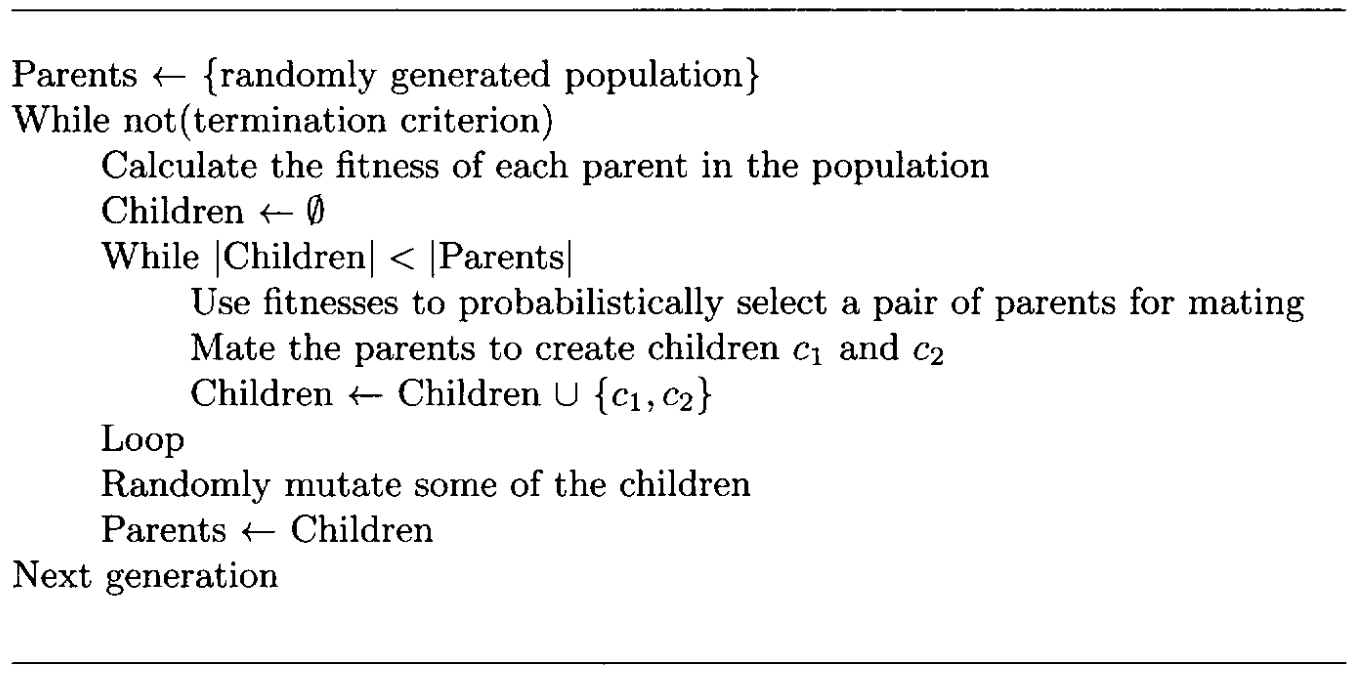
\includegraphics[width=0.5\textwidth]{images/ga_pseudo.png}
\end{figure}

EA insgesamt sind Problem-unabhängig, das heißt, dass wenn es eine geeignete Darstellung der Lösungen und eine geeignete Zielfunktion gibt, kann theoretisch jedes Problem mittels EA optimiert werden. Aus diesem Grund gibt es bei jeden EA ein Element der \textbf{Adaptation}.\par
In Teil 2 sowie in Teile 4 bis 6 kann \textbf{Zufälligkeit} verwendet werden, je nachdem welche Verfahren bzw. ausgewählt werden.\par
In dem Mutation-Teil, eine hoch Wahrscheinlichkeit, um Elemente zu mutieren, heißt viel \textbf{Erkundung} und weniger \textbf{Ausbeutung}, und umgekehrt.

\subsection{Particle Swarm Optimization - PSO}
Particle Swarm Optimization (PSO) ist ursprünglich in \cite{kennedy_pso} und in \cite{shi_pso} präsentiert.\par
PSO ist auf menschlichen sozialen Verhalten basiert. \cite{eberhart_pso} Genauer,  PSO basiert auf der Beobachtung von Gruppen von Individuen, die zusammenarbeiten, um nicht nur ihr kollektives Verhalten in einer bestimmten Aufgabe zu verbessern, sondern auch ihr individuelles Verhalten zu verbessern.\par
Die Grundideen hinter PSO sind folgende:

\begin{itemize}
\item Es gibt eine Menge Partikeln, die sich mit einer beliebigen Geschwindigkeit durch den Suchraum bewegen.
\item Der Suchraum ist in \enquote{Nachbarschaften} mit einer beliebigen gleichen Größe unterteilt.
\item Jeder Partikeln speichert sowohl die beste Position, die sie im Suchraum besucht hat, als auch die beste Position, die ihre Nachbarn erreicht haben.
\item Beide die Partikels beste Position und ihre Nachbarns beste Positionen beeinflussen die Partikels Geschwindigkeit.
\end{itemize}

\begin{figure}[h]
\caption{Wesentlich PSO Algorithmus pseudo-Code. Quelle: \cite{wiley_evolutionary}}
\label{fig:pso_pseudo}
\centering
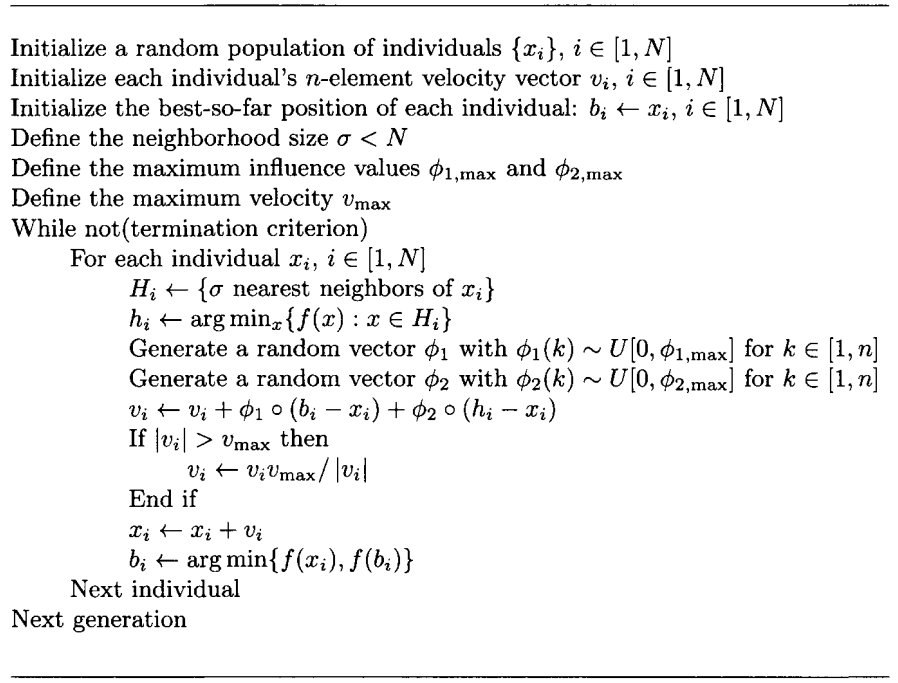
\includegraphics[width=0.5\textwidth]{images/pso_pseudo.png}
\end{figure}

In PSO können die Geschwindigkeiten der ersten Bevölkerung zufällig initialisiert werden. Daher haben wir ein Element der \textbf{Zufälligkeit}.\par
Da die Partikeln die beste bisher erreichte Positionen ihrer Nachbarn kennen müssen, gibt es auch Kommunikation.\par
Die Tatsache, dass die beste bisher erreichte Positionen die Geschwindigkeit der Partikel beeinflussen, zeigt \textbf{Rückmeldung}. In welche Ausmaß wird die Partikel beeinflusst, kann entweder \textbf{Erkundung} oder \textbf{Ausbeutung} fördern.

\subsection{Differential Evolution - DE}
Es wurde erstmals in \cite{storn_de_a} und \cite{storn_de_b} über differential Evolution (DE) diskutiert. Aber die erste vielfach gelesene DE-Veröffentlichung war \cite{price_storn_de}.\par
Im Gegensatz zu fast alle andere EA, DE ist nicht auf der Natur inspiriert. Eine die wichtigste Merkmale der DE ist, dass es einfach ist. Dies Merkmal ist wichtig, da es erlaubt Benutzer aus andere Bereiche (d. h. nicht Informatikern/inen oder Mathematiker/inen), es umzusetzen.\par
Die wesentliche Schritte eines DE Algorithmuses sind die folgende:

\begin{enumerate}
\item Die Bevölkerung eines DE Algorithmus besteht auf Vektoren mit $n$ Elemente. Wo $n$ ist auch die Dimension des Problems. Weiterhin, jeder Vektor selbst stellt eine mögliche Lösung des Problems dar.
\item Zwei Vektoren $x_{r2}, x_{r3} \mid r2 \neq r3$ werden ausgewählt.
\item Die Differenz zwischen $x_{r2}$ und $x_{r3}$ wird berechnet.
\item Die skalierte Differenz wird zu einem dritten Vektor $x_{r1} \mid r1 \notin \{ r2, r3 \}$ addiert. Das wird eine neue mögliche Lösung $v_i$ ergeben.
\item $v_i$ wird mit einem Vektor $x_i \mid i \notin \{ r1, r2, r3 \}$ kombiniert.
\item $x_i$ wird gegen $u_i$ vergleicht und nur der beste wird behaltet.
\end{enumerate}

Abbildung \ref{fig:de_beispiel} zeigt Schritte 2 bis 4 für ein Problem mit 2 Dimensionen. Abbildung \ref{fig:de_pseudo} zeigt einen ganze DE Algorithmus pseudo-Code für $n$ Dimensionen.\par

\begin{figure}[h]
\caption{Grundlegende Idee von DE. Quelle: \cite{wiley_evolutionary}}
\label{fig:de_beispiel}
\centering
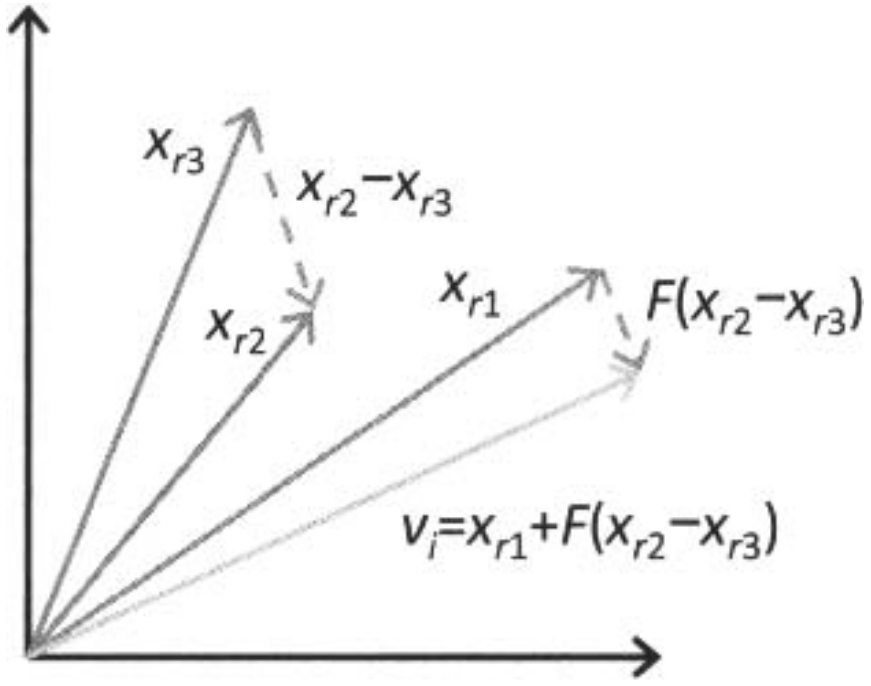
\includegraphics[width=0.5\textwidth]{images/de_beispiel.png}
\end{figure}

\begin{figure}[h]
\caption{Wesentlich DE Algorithmus pseudo-Code. Quelle: \cite{wiley_evolutionary}}
\label{fig:de_pseudo}
\centering
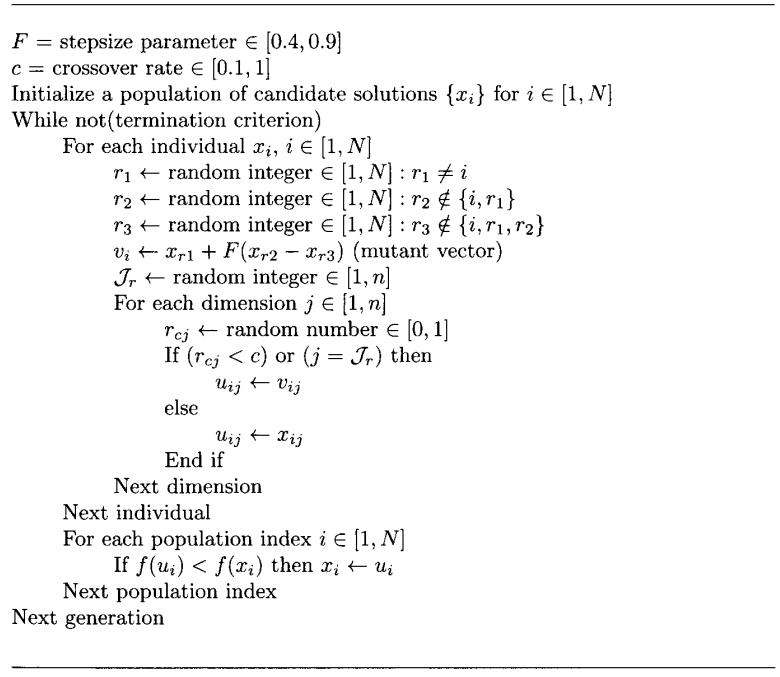
\includegraphics[width=0.5\textwidth]{images/de_pseudo.png}
\end{figure}

Der Algorithmus, den die Abbildung \ref{fig:de_pseudo} beschreibt, ist \enquote{DE/rand/1/bin} genannt und es ist die einfachste Variante der DE Algorithmen. Andere Varianten sind z. B. \enquote{DE/best/1/L}, \enquote{DE/best/2/bin}, \enquote{DE/rand/1/exp},  u. v. a. m.\par
Jedes Teil dieser Namen bezieht sich auf die Verfahren, die für bestimmte Schritte der DE Algorithmen verwendet werden.\par
Zum Beispiel der \enquote{rand/best}-Teil\footnote{\enquote{best} und \enquote{rand} sind nicht die einzige Varianten.} beschreibt wie Vektoren $x_{r1}$ und $x_{r2}$ im 2. Schritt ausgewählt werden. \enquote{rand} bedeutet, dass die Vektoren zufälligerweise ausgewählt werden, während \enquote{best} heißt, dass die beste Vektoren eine höher Wahrscheinlichkeit haben, um ausgewählt zu sein.\par
In \cite{love_u_mex} werden die Leistungen mehrerer Varianten von DE Algorithmen vergleicht.\par
Wenn Vektoren $x_{r1}$ und $x_{r2}$ zufällig ausgewählt werden, gibt es ein Element der \textbf{Zufälligkeit}. Wenn nur die beste Vektoren ausgewählt werden, wird \textbf{Ausbeutung} gefördert. Die Tatsache, dass nur die beste Vektor im 6. Schritt behaltet wird, zeigt \textbf{Rückmeldung}. Die Kombination, die im 5. Schritt stattfindet, könnte auch entweder \textbf{Erkundung} oder \textbf{Ausbeutung} fördern.

%------------------------------------------------

\section{Diskussion}
\lettrine[nindent=0em,lines=3]{D} as größte Vorteil des evolutionären Algorithmen ist, dass es praktisch keine Grenze dafür gibt, wo können sie verwendet werden. Wie vorher gesagt, wenn es eine geeignete Darstellung der Lösungen eines Problems gibt, und eine geeignete Zielfunktion sich definieren lässt, kann jedes Problem mit EA optimiert werden.\par
Eine Nachteil der EA ist, dass eine geeignete Zielfunktion zu definieren ein Problem gleich groß (oder auch größer) als das ursprüngliche erstellen könnte. Eine Möglichkeit, dies zu vermeiden ist das Problem zu teilen. In der Praxis werden oft EA verwendet, um mehrere separate Teile großer komplexer Systemen zu optimieren.\par
Noch ein Nachteil der EA ist, dass die Einstellung des Parametern der Algorithmen könnte auch ein großes Problem darstellen. Die Leistung der Algorithmen ist wirklich davon abhängig, wie die ursprüngliche Bevölkerung initialisiert ist, und was für Werte für die Parametern der Algorithmen ausgewählt werden. Dies ist so ein großes Problem geworden, dass dazu Forschung betrieben wird. Um einige Beispiele zu nennen \cite{pso_tuning_a}, \cite{pso_tuning_b}, und \cite{pso_tuning_c} stellen Verfahren zur Parametereinstellung für PSO vor.\par
EA sollten berücksichtigt werden, immer wenn ein schweres Optimierungsproblem gelöst werden soll. Das bedeutet aber nicht, dass EA sind immer die beste Wahl für den Job; Wenn eine Gebäude oder ein komplexes Transportsystem projektieren werden soll, dann sind EA eine geeignete Werkzeug; Wenn ein komplexe elektrische Schaltung oder ein Computerprogramm entwerfen werden soll, dann können die EA die Aufgabe erfüllen; Aber wenn das Problem jedoch mit klassischen Methoden, entweder analytisch oder numerisch, eine gute genug Lösung bietet, ist es besser, diese Methoden zu verwenden.

%------------------------------------------------

\section{Fazit}

\lettrine[nindent=0em,lines=3]{D} ank der Wachstum des Informatikbereichs und der heutige Rechnerleistung es ist immer mehr möglich, größer und komplexer Systeme zu entwickeln. Dies bringt auch große und komplexe Herausforderungen mit. EA (und KI insgesamt) sind aber gute Werkzeuge um diese neue Herausforderungen zu überwinden.\par
Künftig sollen EA in möglichst immer mehr Bereiche eingeführt worden. Ferner sollen wir weiterhin die Natur als Inspiration betrachten. Sowohl in der Wissenschaft, als auch in der Kunst, hat sich die Natur als die beste Muse erwiesen.

%----------------------------------------------------------------------------------------
%	REFERENCE LIST
%----------------------------------------------------------------------------------------

\renewcommand{\refname}{Quellenverzeichnis}
\bibliographystyle{alpha}

\bibliography{quellenverzeichnis}

%----------------------------------------------------------------------------------------

\end{document}
